\section{Introduction}\label{sec:intro}
Textual program editors are powerful and expressive user interfaces,
so it is perhaps little wonder that they remain dominant decades after the teletype.
However, textual user interfaces are not the best tool for every job.
In particular, there are many
data types for which a non-textual
user interface for expression construction may situationally be more appropriate \cite{Graphite}.

As a simple example, consider a record type
classifying colors using an RGBA encoding:
\begin{lstlisting}[numbers=none]
type Color = { r: Int, g: Int, b: Int, a: Int }
\end{lstlisting}
It is possible to select a particular color by entering
an expression of this type using a text editor:
\begin{lstlisting}[numbers=none]
let bgcolor : Color = { r: 255, g: 178, b: 45, a: 100 }
\end{lstlisting}
The problem is that this user interface for color selection
offers the user no immediate feedback
and limited editing affordances.
It is difficult for the programmer, or anyone subsequently reading or modifying the code, to know which color is represented
and to interactively tweak that color.

Better support for manipulating data of types like these would be particularly helpful for users engaging in
live and exploratory programming in domains like web design, media production,
and data analysis. Indeed, practitioners in domains like these commonly eschew general-purpose programming
in favor of graphical end-user applications, like %
image and video editors and music composition software,
in part because these applications provide domain-specific forms of live feedback and
direct manipulation affordances, e.g. color palettes, visual timelines, and interactive plots.
The trade-off is that these applications have limited support for abstraction and composition.
It is difficult, for example, to bind a
color to a variable for use in multiple locations,
or to transform a sound by passing it through a series of functions,
or to define a function that computes a vector graphic given a set
of parameters (some of them perhaps themselves computed),
or to organize these constructions into modules.
Moreover, it is difficult to add new affordances or to compose
affordances in ways that the application designer did not anticipate,
so users cannot easily make even simple changes like replacing a numeric text box in a color chooser with a slider,
much less more ambitious changes like a new visual interface for expressing geospatial data queries.

This paper aims to resolve the apparent tension between
programmatic and direct manipulation user interfaces by designing a programming system that
is able to surface GUIs for the data types for which
they are useful, while retaining full support for symbolic program manipulation
and the abstraction and composition mechanisms
available in modern general-purpose languages.

\subsection{Background}
\begin{figure*}
  \begin{center}
    \begin{subfigure}[t]{0.5\textwidth}
      \centering
      \vspace{-3.4cm}
      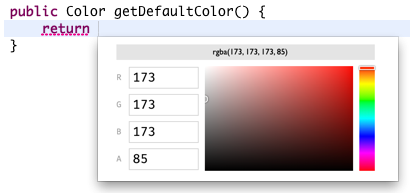
\includegraphics[width=15pc]{graphite-color-palette.png}
    \end{subfigure}\begin{subfigure}[t]{0.5\textwidth}
      \centering
      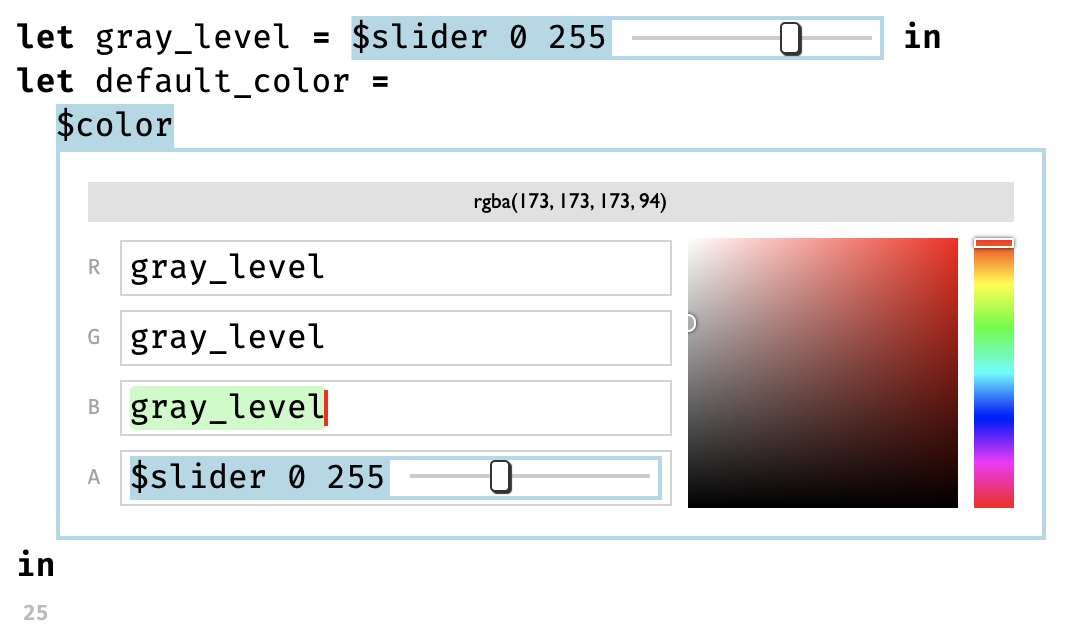
\includegraphics[width=15pc]{slider-color-livelits.png}
    \end{subfigure}
  \end{center}
  \caption{
  (a) This figure, adapted from the prior work of \citet{Graphite},
  shows a Graphite palette associated with the \texttt{Color} class.
  The client can specify the RGBA components only using literal numbers.
  (b) A similar Hazel livelit for colors uses live splices for the RGBA components,
  so the client can enter any Hazel expression.
  In this case, the client has entered a variable, itself defined using a slider livelit, into the RGB
  splices. The A splice is filled directly with a slider livelit.
  The color livelit evaluates splices under its closure to display the
  computed color.
  The value of \li{default\_color} is determined by the livelit via a macro expansion step.}
  \label{fig:color}
\end{figure*}

We are not, of course, the first to seek to integrate direct manipulation user interfaces
into general-purpose programming systems.
Prior work on projectional editing
and active code completion, detailed in Sec. \ref{sec:related-work},
has also considered the problem of entering expressions
of certain types, like \li{Color},
using specialized GUIs integrated into a program editor.
The prior work most closely related to this paper is the {Graphite} system for Java \cite{Graphite},
demonstrated in Fig.~\ref{fig:color}(a).
Graphite allows library providers to associate GUIs, called \emph{palettes}, with types (using Java's class annotations).
Wherever an expression of a type equipped with a palette is needed,
i.e. wherever there is a \emph{hole} of that type in the program,
the programming environment offers the programmer the option, via the code completion menu,
to activate the palette.
Once the interaction is finished, it is the palette's job to generate an
appropriate Java expression to fill the hole.
Figure~\ref{fig:color}(a)\todo{use subfigure?}{}, adapted from this prior work, demonstrates a color palette invoked using Graphite.
When the user presses the \li{Enter} key, the Java expression \li{new Color(0, 0, 128)}\todo{correct code}{} is inserted at the cursor (not shown) and the palette disappears.

\citet{Graphite} extensively evaluated this mechanism.
Most notably, a survey of approximately 450 developers found that
most of these developers viewed the proposed mechanism favorably and stated that they
would use a suitable palette some or all of the time if one was available.%
\footnote{When presented with a color palette,
many participants remarked that they rarely entered colors directly into Java code,
but rather into stylesheets or other files governed by a domain-specific language.
Other palettes, e.g. a palette
that supported regular expression construction and testing, were viewed as more
suitable for Java code.
The mechanisms being considered are suitable both for general-purpose languages
and typed domain-specific languages, many of which can be embedded into modern
general-purpose languages, e.g. Typed CSS in Reason. TODO: CITE}
This survey also solicited a large number of use cases from the survey participants,
which the authors grouped into several broad categories. Notable examples include:
\begin{itemize}
  \item \textbf{graphical elements}, such as brushes, fonts, polygon editors, user interface widgets, and 3D primitives;
  \item \textbf{data analysis primitives}, such as plot setups and database queries;
  \item \textbf{composite data structures} such as matrices, maps, queues, and others for which specialized notation and affordances may be more suitable than general-purpose mechanisms; and
  \item \textbf{data transformations} for which sensory feedback could aid in understanding,
  e.g. audio filters, image transformations, and animations with parameters such as speed and shape.
\end{itemize}

We take the extensive empirical evaluation performed by \citet{Graphite} as sufficient to establish
the utility and broad applicability of a mechanism of this class.

\subsection{Contributions}

Our focus in this paper is on addressing several non-trivial technical
deficiencies that limit both palette providers and palette clients in Graphite.
The system of \emph{live literals}, or \emph{livelits} introduced in
this paper and demonstrated in Fig.~\ref{fig:color}(b) improves upon Graphite
in each of the following ways.
\begin{enumerate}
  \setlength\itemsep{0.5em}
  \item \textbf{Decentralized Extensibility}:
    In Graphite, only one palette can be associated with a type, and this must
    be done at the definition site.
    By contrast, livelit definitions are orthogonal to type definitions.
    Clients invoke livelits explicitly via their names, which are prefixed by the \li{\$} character,
    e.g. \li{\$color} and \li{\$slider} in Fig.~\ref{fig:color}(b).
    We call this \emph{decentralized extensibility}.
  \item \textbf{Persistence}: Graphite's palettes are {ephemeral},
  i.e. they disappear after the initial interaction,
  leaving behind only the generated textual code.
  Consequently, only the programmer that initially enters the expression
  benefits from the feedback and affordances that the palette provides.%
  \footnote{Graphite does include an \emph{ad hoc} mechanism that
  allows palettes to parse the code that is selected in the editor
  when the palette loads, but this requires that each palette implement
  a parser for the subset of Java used in the code that it generates,
  and therefore this mechanism is quite brittle. It is also difficult
  to persist GUI state that is not included in the generated code.}
  By contrast, livelits are persistent. We use a pure functional model-view-update architecture
  (i.e. the Elm architecture\todo{what to cite?}{}) as our GUI framework,
  so only the model needs to be persisted, rather than the full GUI state.
  We use the word ``literal'' rather than ``palette'' because, with persistence, livelits
  operate as graphical literal notation, e.g. list literals.

  \item \textbf{Compositionality}:
  Graphite does not provide any way to {enter subexpressions within a palette}.
  At best, palettes can contain text boxes, but expressions entered into these text boxes
  do not have any editor support (which creates many problems, one of which is that they cannot themselves be generated by palettes).
  This implies that palettes can only reasonably generate {closed expressions}.
  For example, in Figure~\ref{fig:color}(a), the color palette
  is useful only for generating simple color constants.
  By contrast, livelits have first-class support for subexpressions, which we call \emph{splices} (following
  the terminology of \citet{TLMs} who developed reasoning principles for splicing in a strictly textual setting).
  Fig.~\ref{fig:color}(b) demonstrates splicing: the client is able to define a variable, \li{gray\_level},
  to capture the relationship between the red, green, and blue components.
  The client is also able to use a slider inline in the splice governing
  the alpha (A) component.

  \item \textbf{Parameterization}: It is possible to define parameterized families of livelits.
  For example, \li{\$slider} in Fig.~\ref{fig:color}(b) is parameterized by the lower and upper bound.
  Parameters behave like splices, differing in that livelit parameters can be partially applied in
  livelit abbreviations. For example, it is possible to define a livelit named \li{\$percentage}
  that operates as a \li{\$slider} from \li{0} to \li{100} by scoped abbreviation:
  \begin{lstlisting}[numbers=none]
  let livelit $percentage = $slider(0, 100) in ...
  \end{lstlisting}
  Parameterization also underlies the hygiene mechanism, as we will discuss in Sec.~\ref{sec:livelit-definitions}.

  \item \textbf{Liveness}: Graphite's palettes do not have
  access to the run-time environment. By contrast, livelits can evaluate splices
  and therefore provide feedback related to the run-time behavior of the expression being generated.
  For example, in Fig.~\ref{fig:color}(b), the color that is displayed is determined by evaluating the RGBA
  component splices to numeric values.
  Evaluation occurs in a run-time environment (i.e. closure) determined by
  leaving the hole being filled by the livelit temporarily unfilled and then evaluating
  using a two-phased variation on the semantics for incomplete programs developed for Hazel \cite{HazelnutLive}.
  We will see more sophisticated examples later in the paper, including a livelit
  that appears inside a function that is called multiple times, leading to multiple closures that the client can
   select between.
\end{enumerate}

\noindent
\textbf{Outline.} The remainder of this paper is organized as follows. We begin in Sec.~\ref{sec:case-studies} with case studies
involving several non-trivial livelits, focusing on the livelit client's perspective.
In Sec.~\ref{sec:livelit-definitions}, we consider the livelit provider's perspective by detailing the livelit
definition mechanism by example.
In Sec.~\ref{sec:livelit-calculus}, we provide a formal account of the livelit mechanism as a typed lambda calculus.
This calculus formally specifies the essential aspects of livelit definition, representation, expansion,
and run-time closure collection independent of the particularities of GUI framework and other implementation details.
This calculus and the key metatheoretic properties has been mechanized in Agda.
In Sec.~\ref{sec:extensions}, we describe some extensions of the core calculus\todo{what are the extensions?}{}.
In Sec.~\ref{sec:implementation}, we provide a more detailed account of our implementation of livelits within Hazel,
and discuss several implementation details that would need to be considered by other implementations.
In Sec.~\ref{sec:related-work}, we compare livelits to related work.
Finally, we conclude in Sec.~\ref{sec:discussion} with a discussion of some present limitations and future work.